\documentclass[sigconf]{acmart}

\usepackage{graphicx} % For graphics
\usepackage{float} % For graphics placement, et al.
% \usepackage{amsmath} % For formulas (don't need)
% \usepackage{booktabs} % For formal tables (don't need)

\acmConference[CSPB 4502]{CU CSPB 4502 - Data Mining}{Fall 2024}{Boulder, CO, USA}
\acmYear{2024}
\acmMonth{10}

% remove ACM reference format section
\settopmatter{printacmref=false}

% remove copyright section
\renewcommand\footnotetextcopyrightpermission[1]{}

% Meta Information for the document
\title{Detecting Malicious Behaviors on Ethereum}
\author{Hallee Ray}
\affiliation{%
  \department{Computer Science Post Bacc.}
  \institution{University of Colorado - Boulder}
  \city{Boulder}
  \state{Colorado}
  \country{USA}
  \postcode{ZIP code}
}
\email{hara7620@colorado.edu}


\author{BD Tinsley}
\affiliation{%
  \department{Computer Science Post Bacc.}
  \institution{University of Colorado - Boulder}
  \city{Boulder}
  \state{Colorado}
  \country{USA}
  \postcode{ZIP code}
}
\email{beti7384@colorado.edu}

\author{Evan Bean}
\affiliation{%
  \department{Computer Science Post Bacc.}
  \institution{University of Colorado - Boulder}
  \city{Boulder}
  \state{Colorado}
  \country{USA}
  \postcode{ZIP code}
}
\email{evbe5723@colorado.edu}
% \author{Another Author}
% \affiliation{%
%   \institution{Another Institution}
%   \city{City}
%   \state{State}
%   \country{Country}
%   \postcode{ZIP code}
% }
% \email{anotherauthor@example.com}

\begin{document}

% abstract
\begin{abstract}
This project aims to analyze transaction data from the Ethereum blockchain to detect fraudulent or suspicious activities using data mining techniques. By utilizing real-time data and feature engineering, we will develop models that can predict malicious behaviors, identify trends, and detect anomalies in blockchain transactions. We also aim to enhance our dataset by incorporating public interest data from Google Trends and findings from FBI reports. Our final objective is to build a system that can flag potentially fraudulent wallets and predict suspicious activity before it escalates.
\end{abstract}

% keywords
\keywords{Ethereum blockchain, anomaly detection, data mining, prediction modeling, fraud detection, feature engineering, machine learning}

% main content
\maketitle

\section{Problem Statement/Motivation}

We will mine data from the Ethereum blockchain to discover trends in transactions. Through this analysis, we aim to detect fraudulent or scam-like trends involving investment fraud, kiosk scams, and other malicious behaviors. Our goal is to answer several interesting questions related to the relationships between different features of Ethereum transactions. One question we seek to explore is whether there is a correlation between the time of the transaction and the amount of the transaction. This could help us identify patterns regarding the time of day or night during which larger transactions are reported. Intuitively, we suspect that transactions for large amounts occurring outside of normal trading hours may be more likely to be fraudulent.

Another question we aim to investigate is the average time between a new coin going live and its first purchase. Exploring this question could provide insights into potential pump-and-dump activities. For instance, if there is a higher-than-average volume of transactions within the first 24 hours of a coin becoming available for trading, it could drive up the price of the coin, leading to a quick sell-off by investors while the price is artificially inflated.

Additionally, we are interested in the average values of transactions during the lifetime of Ethereum and how they map to early-stage hype. This analysis could help us recognize patterns related to a coin’s overall health in the market. For coins with a history of fraudulent activity, we will examine the general statistics of the transactions that were reported as fraudulent. This investigation could allow us to establish guidelines for identifying transactions that should be flagged as potentially fraudulent.

By analyzing these questions, we aim to gain a deeper understanding of Ethereum transactions and improve our ability to predict whether a transaction is likely to be fraudulent.

\section{Literative Survey}
\subsection{The Literature of Fraud Data and Identification}
Unfortunately, scams and fraudulent activity in cryptocurrency occur frequently and are difficult to monitor due to the anonymous and decentralized nature of cryptocurrency. The Federal Bureau of Investigation (FBI) and the Homeland Defense \& Security Information Analysis Center (HDIAC) have made efforts to monitor and predict fraudulent behavior in cryptocurrency.

"In February 2022, the FBI formed the Virtual Assets Unit (VAU), a specialized team dedicated to investigating cryptocurrency-related crimes" \cite{FBI2023}. In the report, the FBI identified common types of malicious behaviors using cryptocurrencies: investment fraud, recovery schemes, and kiosk scams. Investment fraud is described as malicious actors who encourage individuals to make “investments” in cryptocurrency. The FBI found that losses from cryptocurrency-related investment fraud schemes reported to the IC3 rose from \$2.57 billion in 2022 to \$3.96 billion in 2023, an increase of 53%.

Recovery schemes involve representatives from fraudulent businesses claiming to provide cryptocurrency tracing and promise an ability to recover lost funds. They request an upfront fee for this service and then immediately cease communication with the sender once the funds are received. Kiosk scams are scams where a criminal actor will direct an individual to withdraw cash from their bank and locate and send money via a kiosk or ATM-like machine. In 2023, the IC3 received more than 5,500 complaints reporting the use of cryptocurrency kiosks, with losses over \$189 million.

Knowing the existence of these scams and monitoring statistical metrics regarding cryptocurrency transactions and fraudulent activity is not sufficient to predict and prevent such scams. The Homeland Defense \& Security Information Analysis Center (HDIAC) has employed various real-time predictive machine learning models and on- and off-chain monitoring to detect fraudulent activity. The HDIAC describes the purpose of the off-chain module as preventing fraud before it occurs, whereas the on-chain module utilizes real-time surveillance to detect fraud after it has occurred \cite{HDIAC2023}.
\subsection{The Literature of Formal Fraud Detection Methods}
\subsubsection{Formal Methods}
In a manuscript submitted in August of 2024, Jin et. al from Zhejiang University of Technology, China discuss methods of designing fraudulent action detection system in the Ethereum Blockchain. Noting, as we have, that many forms of fraud require expert systems with subject matter expertise to rule on what seems “irregular” and what does not, Jin suggested using transaction-graph-based methods of anomaly detection to target individual malicious accounts and behaviors. At its core, the methodology is pattern recognition and segregation. The challenge of this approach, however, is gracefully handling complex, frequent, and imbalanced data. As one might expect, some perfectly good actors will trade at a low volume and frequency – consider the armchair cryptocurrency enthusiast, while other good actors will technical capabilities and more personal investment in cryptocurrency might seek out arbitrage, small-margin, or options plays, all of which characteristically “look” very different. To be able to segregate the good from the bad, one must categorize these different behavioral patterns, normalize the weighting that may be associated with high volumes of varying types of trades or traders so that a predictive engine is not overly focused on a majority, but rather equally focused on varying patterns.
Within graph analysis, we will follow and expand upon the methodologies presented by Jin. This will be discussed in greater detail below.
\cite{EnhancingEthereumFraudDetection}

\section{Proposed Work}

The work that we will need to perform in order to progress through this project involves \textbf{data preprocessing}, \textbf{exploratory data analysis}, \textbf{feature engineering}, \textbf{anomaly detection}, and \textbf{prediction modeling}.

\subsection{Data Preprocessing}
For data preprocessing, there are two steps that will need to be completed: \textbf{data cleaning and preparation}, and \textbf{normalization and standardization}. This can be achieved by handling any missing values in a variety of ways, such as:
\begin{itemize}
    \item \textbf{Dropping records} that cannot be filled in through integrating multiple sources.
    \item \textbf{Filling in missing values} with a predetermined default value.
    \item \textbf{Imputing missing values} based on similar records.
\end{itemize}
Additionally, the fields of each feature will need to be analyzed and converted to the correct \textbf{data types} and formats.

\subsection{Exploratory Data Analysis}
\textbf{Exploratory data analysis} will help us uncover inter- and intra-feature relationships. \textbf{Univariate analysis} and \textbf{visualization} will allow us to identify outliers and anomalous values. Visualizing a \textbf{heatmap} of the correlations between features will allow us to understand general trends between features.

\subsection{Feature Engineering}
An important step in feature engineering is deriving new attributes, such as:
\begin{itemize}
    \item New attributes for \textbf{transaction time intervals}, including \textbf{in-degree} and \textbf{out-degree} for sender and recipient addresses.
    \item Grouping various features according to their \textbf{transaction patterns} and frequency.
\end{itemize}

\subsection{Anomaly Detection}
One of the main objectives of this project is to detect anomalies that could potentially be fraudulent. Statistical methods such as \textbf{Z-score} and \textbf{Percentile-Based Detection} can be utilized to isolate transaction values of unusually high or low values. We can use the same methods to identify feature values that fall well outside the standard range.

\textbf{Distance-based methods} can be employed to detect anomalies. By defining several dimensions such as \textbf{time\_between\_transactions} and \textbf{gas\_price} (based on gas and value), we can measure the distance between transactions and compare the record to its nearest neighbors using the \textbf{K-Nearest Neighbors (KNN)} methodology. Outliers here will also show interesting trends. 

Using \textbf{K-means Clustering}, we can determine address behavior based on clusters by transaction activity, including:
\begin{itemize}
    \item \textbf{Total transaction value}
    \item \textbf{Transaction frequency}
    \item \textbf{Gas usage}
\end{itemize}
Addresses that fall into distant clusters or small clusters could indicate suspicious behavior.

\subsection{Prediction Modeling}
Finally, we propose \textbf{prediction modeling}. Using statistics defined in \textbf{FBI’s Internet Crime Complaint Annual Reports}, we will enhance our dataset by incorporating fraud patterns from FBI statistics, such as:
\begin{itemize}
    \item Prevalence of specific fraud types.
    \item Trends in fraudulent activity over time.
\end{itemize}
Labeling the historical transaction data and using a \textbf{Random Forest} supervised machine learning model will help us discover potential fraudulent activity. Using real-time Ethereum data and our predictive models, we aim to \textbf{predict and mark transactions as potentially fraudulent} as they occur.

\section{Dataset}

The datasets that we will utilize for this project are an Ethereum ledger that provides real-time transaction data showing transaction type, the sender and recipient wallets, and the transaction amount via API integration \cite{etherscan}. Additionally, we contrast our dataset with maps of public interest in specific Ethereum-built cryptocurrencies using Google Trends \cite{googletrends}. Finally, we will compare our results to FBI findings to determine if we can detect trends before complaints of fraudulent activity using the FBI Fraud Report \cite{FBIFraudReport2023}.

\section{Evaluation Methods}

To quantitatively evaluate the performance of our fraud detection models, we will employ several metrics and methods:

\subsection{Performance Metrics}
We will assess model performance using standard classification metrics such as:
\begin{itemize}
    \item \textbf{Accuracy}: The ratio of correctly predicted instances over the total instances.
    \item \textbf{Precision and Recall}: Critical in fraud detection, precision measures the fraction of actual frauds in the predicted fraud cases, while recall measures the fraction of actual frauds correctly identified. The \textbf{F1-Score}, a harmonic mean of precision and recall, will also be calculated to balance both.
    \item \textbf{ROC Curve \& AUC}: We will use the ROC curve to visualize the trade-off between true positive and false positive rates and calculate the AUC as a quantitative measure of model discrimination.
\end{itemize}

\subsection{Cross-Validation}
We will perform \textbf{k-fold cross-validation} to ensure that our model's performance generalizes well across different subsets of data. This will mitigate overfitting and provide more robust performance metrics.

\subsection{Confusion Matrix}
A \textbf{confusion matrix} will be generated to break down our predictions into true positives, false positives, true negatives, and false negatives. This allows us to analyze misclassifications in more detail.

\subsection{Threshold Tuning}
By adjusting the \textbf{decision threshold}, we will explore how varying thresholds impact precision and recall, allowing us to tune the model based on the relative costs of false positives and false negatives.

\subsection{Anomaly Detection Metrics}
For anomaly detection, we will calculate \textbf{Z-scores} and use \textbf{distance-based metrics} (e.g., K-Nearest Neighbors) to measure how well the model isolates outliers from the normal transaction patterns.

\subsection{Scalability and Time Complexity}
We will evaluate the \textbf{time complexity} of our models and their ability to scale by testing performance on progressively larger subsets of Ethereum transactions.

\subsection{Feature Importance}
Using a \textbf{Random Forest} model, we will assess the importance of various features (e.g., transaction amount, gas price, time intervals) in predicting fraudulent behavior. Feature importance scores will be used to identify the most impactful features.

\subsection{Baseline Comparison}
We will compare the performance of our models against simpler baselines such as logistic regression, measuring improvements in precision, recall, and AUC over the baseline models.

\subsection{Statistical Significance}
We will conduct \textbf{paired t-tests} and \textbf{ANOVA tests} to determine whether improvements in performance metrics between different models are statistically significant.

\section{Tools}

The programming language that we will use for this project is \textbf{Python}, the beloved language for data science projects. It has a vast ecosystem of libraries for data analysis and integrates well with third-party services. Two useful libraries for our objectives include \textbf{SciPy} and \textbf{NumPy}. Both extend Python to include a range of computing tools to handle matrix operations, statistical analysis, optimization, and signal processing. Additionally, the \textbf{Pandas} library will be necessary in our exploration of the data due to its ability to handle structured datasets. It will be useful in most steps of this project but will especially excel in data cleaning, EDA, and feature engineering.

Due to the size of the dataset, we may encounter some limitations with Pandas’ processing speed. Due to the size of the Ethereum blockchain ledger, we will likely be viewing and previewing our work within small time frames to take advantage of Python and Pandas processing power alone. However, when evaluating larger time frames of Ethereum transactions, \textbf{Dask} will be necessary to parallelize Python processing.

Visualization libraries such as \textbf{Matplotlib}, \textbf{Seaborn}, and \textbf{Plotly} will be greatly helpful in our data exploration and performance analysis. Data visualization will be necessary to display outliers and trends we uncover. Matplotlib will be useful for rudimentary visualizations, but we will likely reach for Seaborn for more control over aesthetics and Plotly for interactive visualizations.

\textbf{GitHub} will be a necessary tool for this project, both from a grading perspective and as a way to manage multiple contributors to the same codebase by offering a single source of truth, backups, and trackable changes. Admittedly, the task for \textbf{Snowflake} may be beyond the need for this project, but due to the large volume of data in evaluating Ethereum transactions, we may need more scalability than our standard configuration.

\section{Milestones}
\textbf{Milestone 0: Proposal (October 14)}\\
This encompasses parts 1 and 2 of the project requirements. This integrates any peer or instructor feedback from our initial proposal in order to finalize and improve our project proposition.

\textbf{Milestone 1: Pull Dataset \& Data Cleaning (October 18)}\\
In this milestone, we determine the specific windows of Ethereum transactions we will use for the project and clean them in order to successfully employ our data mining objectives.

\textbf{Milestone 2 \& 3: EDA \& Feature Engineering (October 25)}\\
This milestone will allow us to gain insights into the dataset and uncover important information regarding the features. This milestone is a crucial step toward uncovering patterns and relationships between features.

\textbf{Milestone 4: Progress Report (October 28)}\\
As required by the course, this will be a mid-project check-in as defined in part 3 of the project requirements. This will be a good chance for us to review our progress, review our plan, and reassess our goals.

\textbf{Milestone 5: Anomaly Detection (November 8)}\\
This milestone is another important step toward project completion. By this point, we should all have a decent understanding of the data and which attributes are most implicated in fraudulent transactions, and we can shift focus to understanding which metrics would indicate suspicious activity.

\textbf{Milestone 6: Prediction Modeling \& Analysis (December 2)}\\
Our goal to implement prediction modeling is contingent upon the successful completion of milestone 5. This milestone generally encompasses how we could apply the results of data mining in practice.

\textbf{Milestone 7: Final Report (December 9)}\\
As required by the course, this final report will highlight our procedures, findings, and next steps for this project. It will provide an opportunity to reflect on our processes, what did and did not work well, and provide an overview of our understanding of the material.


\section{Proposal Review}
\subsection{Milestones}
Two additional milestones not included in the project proposal, but are required for the course are added:

\textbf{Milestone 8: Presentation (December 9)}\\
As required by the course, this the final presentation of our findings. Originally omitted in the project proposal.

\textbf{Milestone 9: Project \& Code Description (December 9)}\\
As required by the course, this final code update for the project along with links to presentation, final report and outline of our findings. Originally omitted in the project proposal.

\section{Milestones Completed}
\textbf{Milestone 0: Proposal}\\
This was the prior deliverable and was completed October 14, 2024.

\textbf{Milestone 1: Pull Dataset \& Data Cleaning}\\
This milestone proved more challenging than anticipated. Ethereum transaction data is abundant and accessible, but only through paid third party services or solutions that require storage well beyond the common size on typical home laptops and computers. We initially worked with a sample dataset of 500 transactions, but knew the findings would not be adequate for later milestones. We used the sample dataset for data cleaning purposes. We opted for a paid service for streaming access to pull approximately 140,000 records daily, until our fetch limits are reached. Through this, we can select a high degree of transactions from specific windows to validate our findings and develop and train a prediction model.

Due to the high degree of validation in a blockchain transaction, we found the values to be high fidelity and trustworthy. As Ethereum evolves, new attributes are added to each transaction and we were able to remove several null value attributes that were added in the London Hard Fork update \cite{LondonHardfork} (integrated August 2021) and the Proto-Danksharding update \cite{ProtoDanksharding} (integrated March 2024). Noting that we will need to adequately include these attributes in windows that occur after the update timestamp, for the initial portion of our work we cleaned these features.

Completed October 24, 2024.

\textbf{Milestone 2: EDA}\\
Completed October 27, 2024.

\textbf{Milestone 4: Progress Report}\\
This is self-referential as this progress report correlates to this milestone. Completed October 28, 2024.

\section{Milestones Todo}
\textbf{Milestone 3: Feature Engineering (October 25)}\\
Slated to be completed by October 25, we are running behind schedule completing this milestone. However, due to high degree of fidelity in the dataset, we believe we can make up for lost time
\textbf{Milestone 5: Anomaly Detection (November 8)}\\
\textbf{Milestone 6: Prediction Modeling \& Analysis (December 2)}\\
\textbf{Milestone 7: Presentation (December 9)}\\
\textbf{Milestone 8: Final Report (December 9)}\\
\textbf{Milestone 9: Project \& Code Description (December 9)}\\

\section{Results so far}
\subsection{Correlations}
We found that the correlation matrices fail to uncover interesting correlations between attributes, specifically that transaction value is not strongly correlated with any one feature. Our preliminary feature correlation matrix, shown in Figure~\ref{fig:m4CorrelationMatrix}, reveals intuitive correlations, such as \texttt{block\_number} being strongly correlated with \texttt{transaction\_month}. Additionally, there is a strong negative correlation between \texttt{transaction\_month} and \texttt{transaction\_day}, which suggests temporal clustering of certain types of transactions.

\begin{figure}[h]
    \centering
    \includegraphics[width=0.8\linewidth]{m4-correlation-matrix.png}
    \caption{Correlation matrix of features showing intuitive correlations.}
    \label{fig:m4CorrelationMatrix}
\end{figure}



\subsection{Gas distributions}
Furthermore, tracking \texttt{gas} (the computational effort required to execute a transaction) is an interesting attribute to examine in correlation with transaction value. A high transaction value paired with low gas may reveal unique patterns, as could the inverse. In our initial EDA, we found no strong correlation between \texttt{gas} and \texttt{value}.

We created several distributions of gas-related values, examining both \texttt{gas usage} (the total computational effort required for a transaction) in Figure~\ref{fig:gasUsage} and \texttt{gas price} (the amount a wallet is willing to pay to expedite transactions) in Figure~\ref{fig:gasPrice}.

\begin{figure}[H]
    \centering
    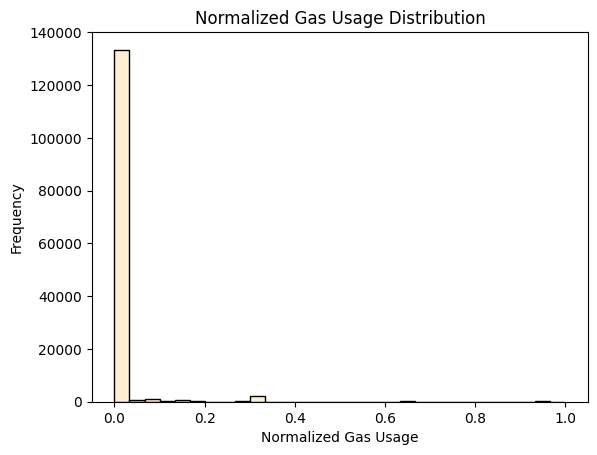
\includegraphics[width=0.8\linewidth]{M4-normalized-distro-gas.png}
    \caption{Distribution of gas usage, showing a high frequency in low gas prices. The outliers may reveal valuable insights.}
    \label{fig:gasUsage}
\end{figure}

\begin{figure}[H]
    \centering
    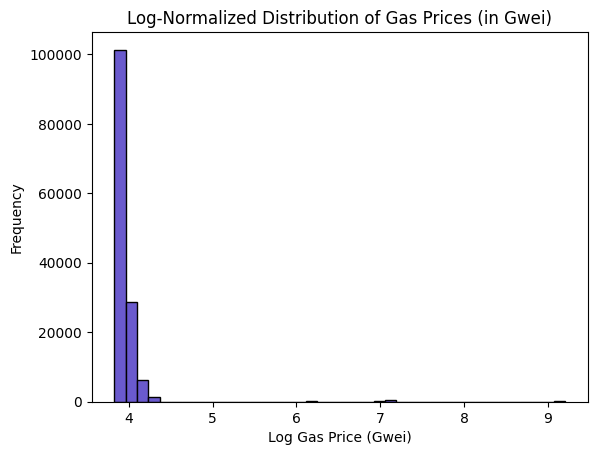
\includegraphics[width=0.8\linewidth]{M4-normalized-distro-gas-price.png}
    \caption{Distribution of gas price, showing a high frequency in low gas prices. Wallets paying significantly more for faster transactions could indicate interesting trends.}
    \label{fig:gasPrice}
\end{figure}

\subsection{Timeplot}
While not directly useful, a time plot of transactions over time in Figure~\ref{fig:timePlot} demonstrates how a brief period represents approximately \( \approx 139,000 \) transactions.

\begin{figure}[H]
    \centering
    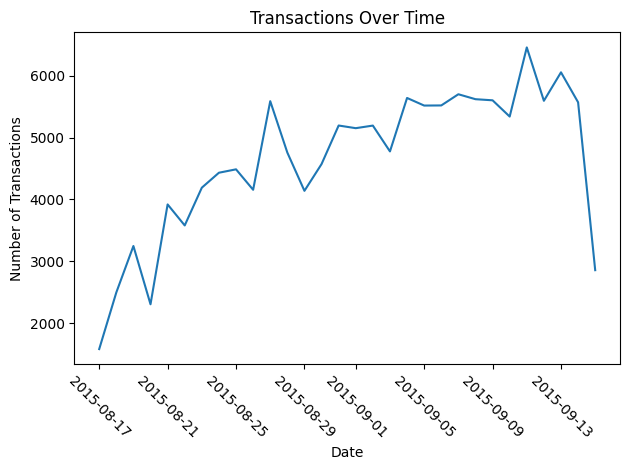
\includegraphics[width=0.8\linewidth]{M4-transactions-timeplot.png}
    \caption{Daily transactions between August 17, 2015, and September 13, 2015.}
    \label{fig:timePlot}
\end{figure}

\subsection{Active wallets}
Identifying the most active senders and receivers is highly informative. As mentioned earlier, fraud may occur within the margins (somewhere between the most and least frequent transactors). By identifying high-traffic vendors or entities, we can remove valid businesses from the dataset or magnify their holdings if they appear compromised. Figure~\ref{fig:activeSenders} shows the most active senders, and Figure~\ref{fig:activeReceivers} shows the most active receivers.

\begin{figure}[H]
    \centering
    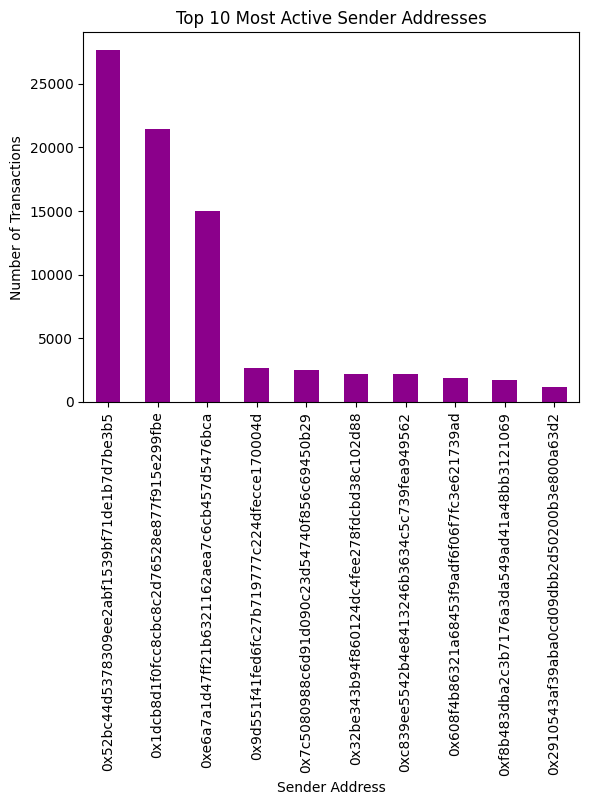
\includegraphics[width=0.8\linewidth]{M4-active-sender.png}
    \caption{10 most active sender wallets.}
    \label{fig:activeSenders}
\end{figure}

\begin{figure}[H]
    \centering
    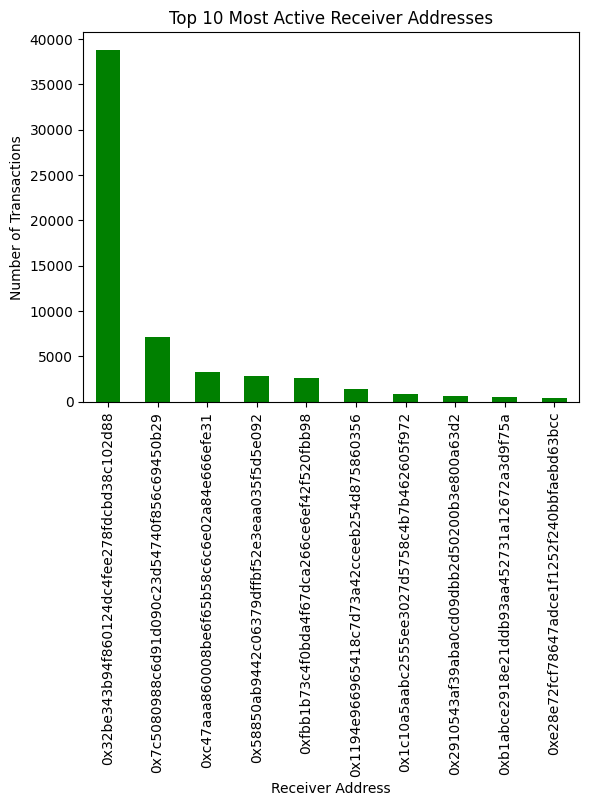
\includegraphics[width=0.8\linewidth]{M4-active-receiver.png}
    \caption{10 most active receiver wallets.}
    \label{fig:activeReceivers}
\end{figure}

\subsection{Nonce distribution}
We have also discovered the importance of the \texttt{nonce} attribute, which increments for each wallet with every transaction. We can use this to track wallets with a high degree of transactions, even if many of them occurred before the start of our observed window. This also allows us to identify wallets completing their first transaction. We believe both the maximum and minimum \texttt{nonce} values within a given window will reveal interesting trends.

Examining the nonce distribution reveals a high degree of first-time senders, as shown in Figure~\ref{fig:nonceDistro}. This pattern may indicate a trend in creating "burner" wallets to avoid detection. Closer analysis of low-nonce transactions could provide more insight.

\begin{figure}[H]
    \centering
    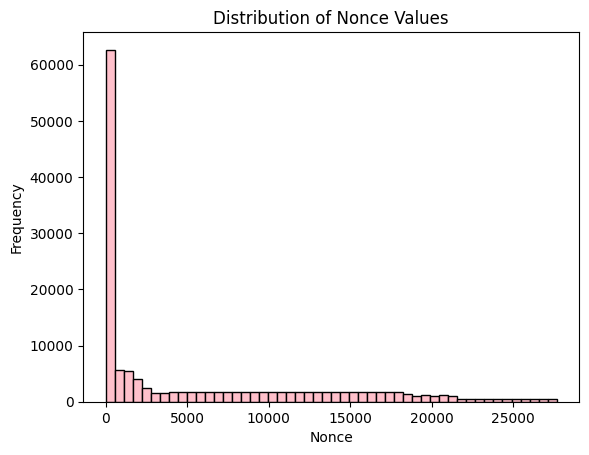
\includegraphics[width=0.8\linewidth]{M4-nonce-distro.png}
    \caption{Distribution of nonce values, highlighting a high proportion of first-time senders.}
    \label{fig:nonceDistro}
\end{figure}


\bibliographystyle{ACM-Reference-Format}
\bibliography{references} 

\end{document}